%%==================================================
%% chapter03.tex for SJTU Master Thesis
%% Encoding: UTF-8
%%==================================================

\chapter{数据库驱动认知无线电网络中的轨迹跟踪攻击与保护}
\label{chap:mobile}

\section{对认知用户轨迹跟踪攻击}
近年来研究者们发现,对于移动的用户,仅仅保护其位置隐私是不够的,因为对位置隐私的保护并不一定能够保证移动对象的轨迹隐私不被泄露。移动对象的原始轨迹暴露可能导致个人兴趣爱好以及行为模式等隐私信息泄露。比如,通过对轨迹数据的分析,攻击者不仅能够发现移动用户正在什么位置,还能够分析出移动对象的家庭住址、工作地点等私密信息。

在数据库驱动认知无线电网络中,静止用户之间的频谱共享能够较好地实现,但是当网络中存在移动用户时,如何较好地实现对主用户的保护以及如何根据移动用户位置计算频谱相关信息成为更具挑战性的问题\cite{min2011opportunistic}。文献\cite{gao2014supporting}提出一种基于概率的共存模型。数据库通过对认知用户之间的互相干扰来优化频谱分配方案,认知用户根据位置的不确定性对可能存在的干扰进行优化来确定位置更新的频率。然而无论采用何种共存模型,在可用频谱查询过程中,认知用户与数据库之间交互的信息都会导致轨迹隐私的泄露。本节对数据库驱动认知无线电网络中移动用户的轨迹隐私泄露及保护方法进行了研究。因为考虑到网络中的主用户大多为静止的,否则数据库计算频谱可用信息的复杂度将相当高,所以本节只考虑存在移动认知用户而主用户静止的情况下,攻击者对移动认知用户的轨迹跟踪攻击。


基于第\ref{chap:fixed}章的工作模型,我们依然假设认知用户采用了文献\cite{gao2013location}中的位置盲化方案,即在不直接获取认知用户的位置信息的前提下,对移动的认知用户轨迹进行跟踪。对移动用户的轨迹跟踪可以视为一个运动目标跟踪问题。目标跟踪问题中一种比较常用的是搜索方法。在搜索方法中,可以直接对场景中的所有内容进行匹配计算,寻找最佳匹配位置,但这种方法需要处理大量的冗余信息,运算量比较大并且不是特别必要。然而采用一定的搜索算法对未来时刻目标的位置状态进行估计假设,并指定搜索规则,则可以很大程度上缩小目标搜索范围,这具有非常重要的意义。比较常用的方法是预测运动物体下一时刻可能出现的位置,在其相关区域内寻找最优点。

递归贝叶斯估计是进行运动物体跟踪和预测的一种常用方法。递归贝叶斯估计方法\cite{bergman1999recursive}可用于估计隐马尔可夫模型中\cite{hmm}隐状态出现的概率。隐马尔可夫过程是一种统计模型,用来描述一个含有隐含未知参数的马尔可夫过程,其主要用途是从可观察的参数中确定该过程的隐含参数,然后利用这些参数来作进一步的分析,例如模式识别。图\ref{fig:hmm}简单描述了一个隐马尔可夫过程。


\begin{figure}[!htp]\label{fig:hmm}
  \centering
  \includegraphics[width=0.8\textwidth]{figures/chap5/hmm}\bicaption[fig:hmm]{隐马尔可夫模型}{隐马尔可夫模型}{Fig}{Hidden Markov Model}
\end{figure}

设$X=(x_{0},x_{1},...,x_{n})$是隐马尔可夫模型中的一系列隐状态,$Z=(z_{1},z_{2},...,z_{n})$表示一系列可观察状态。
设$Z_{k}$代表联合事件$z_{1},z_{2},...,z_{n}$。基于马尔可夫假设,隐马尔可夫过程中所有状态的概率分布可表示为:
\begin{equation}\label{eq:combination}
p(x_{0},...,x_{k},Z_{k})=p(x_{0})\prod_{i=1}^k{p(z_{i}|x_{i})p(x_{i}|x_{i-1})}
\end{equation}

基于公式\ref{eq:combination},我们可以将递归贝叶斯估计方法中的预测过程写为:
\begin{equation}\label{eq:predict}
p(x_{k}|Z_{k-1})=\int p(x_{k}|x_{k-1})p(x_{k-1}|Z_{k-1})dx_{k-1}
\end{equation}

将更新过程写为:
\begin{equation}\label{eq:update}
p(x_{k}|Z_{k})=\frac{p(z_{k}|x_{k})p(x_{k}|Z_{k-1})}{p(z_{k}|Z_{k-1})}
\end{equation}

为使用上述方法实现对隐状态的预测,我们需要计算$p_{z_{k}|x_{k}}$和$p(x_{k}|Z_{k-1})$两个概率。在对数据库驱动认知无线电网络中移动的认知用户进行轨迹跟踪时,隐状态$x_{i}$代表认知用户的移动轨迹,可观察状态$z_{i}$代表认知用户上报给数据库的使用频道和相应发射功率。我们需要为$x_{k}$与$z_{k}$以及$x_{k}$与$x_{k-1}$建立关联。连续两个隐状态之间的关联可由公式\ref{eq:hidden-states}表示:

\begin{equation}\label{eq:hidden-states}
x_{k}=f(x_{k-1})+v_{k}
\end{equation}

第$k$个时刻的隐状态和观察状态之间的关联可由公式\ref{eq:observed-states}表示:

\begin{equation}\label{eq:observed-states}
z_{k}=h(x_{k})+w_{k}
\end{equation}

这里的函数$f(\cdot)$和$h(\cdot)$是确定性函数,$v_{k}$和$w_{k}$是服从高斯分布的系统随机附加噪声。对移动认知用户的移动路线进行推断可以看成是一种目标跟踪问题。在目标跟踪问题里,$x_{k}$是目标移动信息,由位置$loc_{k}$和速度$vel_{k}$两个分量构成。前者为欧氏空间中的一个点,代表目标当前位置;后者为一个二维速度向量,表示当前目标速度值和运动方向。$z_{k}$代表认知用户接收到的可用频道和相应的允许发射功率,它是关于认知用户与主用户之间相对距离的函数,我们可以根据最大传输功率函数进行计算。

为描述$x_{k}$和$x_{k-1}$之间的关系,我们可以采用熟知的离散时间运动公式\cite{bar2004estimation}来表示:
\begin{equation}
x_{k}=F \cdot x_{k-1} + v_{k}
\end{equation}

在上式中,$F$为时间矩阵,可表示为:
\begin{equation}       %开始数学环境
F=
\left(                 %左括号
  \begin{array}{cc}   %该矩阵一共3列,每一列都居中放置
    1 & T\\  %第一行元素
    0 & 1\\  %第二行元素
  \end{array}
\right)                 %右括号
\end{equation}

$v_{k}=(v_{k}^{1},v_{k}^{2})^{T}$是加性的白噪声向量,其均值$E(v_{k})=0$,协方差矩阵为:
\begin{equation}
\sum = E(v_{k}v_{k}^{T})=
\left(                 %左括号
  \begin{array}{cc}   %该矩阵一共3列,每一列都居中放置
    \frac{1}{3}T^{3} & \frac{1}{2}T^{2}\\  %第一行元素
    \frac{1}{2}T^{2} & T\\  %第二行元素
  \end{array}
\right)                 %右括号
\sigma
\end{equation}

上式中$\sigma$是噪声强度,$T$是两次查询之间的时间间隔。因为考虑到函数$f(\cdot)$和$h(\cdot)$不是线性函数,因此我们采用粒子滤波(Particle Filter)\cite{arulampalam2002tutorial}方法来进行目标跟踪。

粒子滤波是指通过寻找一组在状态空间中传播的随机样本来近似的表示概率密度,用样本的均值代替积分运算,进而获得系统状态的最小方差估计的过程。粒子滤波算法起源于蒙特卡罗方法\cite{hastings1970monte},它是利用粒子集来表示概率分布,可以用在任意形式状态空间模型上,核心思想是通过从后验概率中抽取的随机状态粒子来表示其分布情况,是一种顺序重要性采样法。我们参照文献\cite{bahrak2013ex}提出的粒子滤波方案,在数据库驱动认知无线电环境中设计一种基本的跟踪移动认知用户的算法,其详细步骤见算法\ref{alg:pf}。

\begin{lstlisting}[language={C}, caption={基于粒子滤波的移动用户轨迹跟踪算法}]
输入:认知用户的频谱使用记录S=$(ch_{1},P_{1}),(ch_{2},P_{2}),...,(ch_{k},P_{k})$
输出:认知用户的轨迹信息,包含位置和速度
初始化:设定粒子数量$N_{P}$及初始权值
    
for 所有N_{P}个粒子$i$
    $\omega_{0}^{i}=\frac{1}{N_{P}}$
k=1
while 没有到达预先设定的终止条件 do
    观察到第$k$次事件:$(ch_{i}^{k},P_{i}^{k})$
    T = 第$k$次事件与第$k-1$次事件之间的时间间隔
    重采样:
      根据粒子的权值$\omega_{1},...,\omega_{N_{P}}$进行重要性采样
       依概率序列$(\omega_{k-1}^{1},\omega_{k-1}^{2},...,\omega_{k-1}^{N_{P}})$从粒子序列中采样,重复$N_{P}$次
    预测:
      for 所有的粒子$Par_{1},...,Par_{N_{P}}$ do
           计算运动信息$x_{k}^{i}$:
           $loc_{k}^{i} = loc_{k-1}^{i} + T \times vel_{k-1}^{i} + v_{k}^{1}$
           $vel_{k}^{i} = vel_{k-1}^{i} + v_{k}^{2}$
           $x_{k}^{i} = (loc_{k}^{i},vel_{k}^{i})$
       end for
    更新:
      for 所有的粒子$Par_{1},...,Par_{N_{P}}$ do
           计算粒子权值:
           $\omega_{k}^{i}=Pr(z_{k}|x_{k}^{i})$ = 
           $
           \begin{cases}
           0  \quad z_{k} \neq h(x_{k}^{i})\\
           1  \quad z_{k} = h(x_{k}^{i})
           \end{cases}
           $  
        end for
     粒子权值归一化:
       $\omega_{k}^{i} = \frac{\omega_{k}^{i}}{\sum_{i=1}^{N} \omega_{k}^{i}}$
end while
              
\end{lstlisting}\label{alg:pf}

在算法\ref{alg:pf}中,我们在初始化时使用一个包含有足够多随机分布的粒子来对移动认知用户的位置及速度信息进行估计。在粒子滤波的过程中,每一轮分为重采样、预测和更新三个步骤。重采样时根据上一轮更新步骤中计算出的各粒子的权值进行重要性采样,即只在权值不为0的粒子周边进行采样。在预测阶段,根据预先猜测的粒子运动信息的大致情况来对各粒子的位置和速度进行估算。在更新阶段,若粒子位置符合当前上报的可用频谱单元,则将其权值更新为1,否则权值更新为0。最后将所有粒子的权值进行归一化并用于下一轮的重采样。具体地讲,假设从后验概率$Pr(x_{k-1}|Z_{k-1})$中随机采样$N_{P}$个粒子,我们将这些粒子表示为$\hat{x}_{k-1}^{i},1 \leq i \leq N$。在预测阶段,根据公式\ref{eq:hidden-states}在后验粒子$\hat{x}_{k-1}^{i}$的基础上生成先验粒子$x_{k}^{i}$,即

\begin{equation}
x_{k}^{i} = f_{k-1}(\hat{x}_{k-1}^{i}) + v_{k-1}^{i}
\end{equation}

这里$v_{k-1}^{i}$表示从系统噪声的概率分布中随机抽取的样本。这个过程相当于从创建了先验概率$Pr(x_{k}|Z_{k-1})$中的采样。为了使用观察状态$z_{k}$对粒子状态进行更新,我们为每个粒子计算权值$\tilde{\omega}_{k}^{i}$。这个权值是观察状态的似然,即

\begin{equation}
\tilde{\omega}_{k}^{i} = Pr(z_{k}|x_{k}^{i})
\end{equation}

然后权值需要进行归一化,即
\begin{equation}
\omega_{k}^{i} = \frac{\tilde{\omega}_{k}^{i}}{\sum_{j=1}^{N}\tilde{\omega}_{k}^{i}}
\end{equation}

基于每个粒子的归一化权值,在下一轮重采样时根据相应的权值来创建新的粒子集$\hat{x}_{k}^{i}$,使得对于所有的$i,j$,满足$Pr(\hat{x}_{k}^{i} = x_{k}^{i}) = \omega_{k}^{j}$。
也就是说,每一次采样都是根据粒子的归一化概率进行的,将此过程重复$N_{P}$次,即完成了$N_{P}$个粒子的重采样。

在实际情况下,按照FCC的规定,移动用户每次移动超过100米,则必须要重新查询可用频谱情况以避免对主用户产生干扰,持续移动的认知用户必将频繁地查询数据库。因此以上算法在用户不断移动时能够收集足够多的频谱使用报告消息来实施攻击。

\section{轨迹跟踪攻击的解决方案}

在传统的LBS中,第\ref{chap:related_work}章所述的几种方法一般能够取得一定效果。但是数据库驱动认知无线电网络中用户轨迹跟踪问题与传统的基于位置服务网络中轨迹跟踪问题不同,好奇的数据库可以以频谱使用信息这类旁道信息作为依据来实施推理,而且数据库驱动认知无线电网络中的用户身份标识在注册后无法改变,因此如何防止轨迹跟踪成为一个具有挑战性的问题。在静止认知用户的位置推断攻击中,我们总结了两种导致隐私泄露发生的事件:功率受限和频道切换。移动的用户面临与之相似的泄露方式但却不完全相同。为尽量保护移动用户的轨迹隐私不被泄露,我们仍然将重点放在如何提高攻击者攻击结果的误差距离上面。下面我们考虑如下几种可能发生的情况。

\begin{enumerate}

\item 若某个时刻用户使用频道的功率受限,则可以推断此刻认知用户的位置范围大致在一个圆环型区域,从而在下一轮采样时可根据重要性的变化从而对可能区域周边进行重点采样。这种情况可以导致对跟踪目标运动信息不确定性减小。

\item 若某两个连续的频谱报告消息中频道相同,但允许发射功率变大,则用户持续使用该频道不会导致轨迹信息泄露。若频道相同且发射功率变小,则会面临与功率受限相同的隐私泄露风险。

\item 若某两个连续的频谱报告中认知用户切换了频道,由于相邻两次查询之间认知用户移动的距离不会太远,则攻击者可以在很大程度上认定认知用户处于两个频道的相应功率覆盖范围的交集区域,这也会导致运动信息不确定性减小。

\item 若一个认知用户在其移动范围内可以一直使用一个固定的频道而且该频道的允许发射功率不变,那么针对上一节提出的攻击方法,我们可以通过选择最合适的频道来在最大程度上减小认知用户轨迹信息的泄露。

\end{enumerate}

根据以上分析,我们可以知道,最好的情况是认知用户能够在其移动的轨迹上持续使用相同的频道,且允许发射功率越大越好。于是我们提出如下的频谱查询和选择策略:

(1)在可用频谱请求阶段,用户采用第\ref{subsec:privacy-preserving}节提出的基于$k$-anonymity的查询方式,即同时查询周边大小为$K_{Q} \times K_{Q}$的区域$B$上的可用频谱信息。在接下来的频道选择阶段,认知用户可以根据这些信息来选择在其移动轨迹上最优的频道。

(2)在频谱选择阶段,用户维护一个关于所有频道的优先级列表:$U=(u_{1},u_{2},...,u_{C})$,每个频道$ch_{k}$的优先级可以表示为:

\begin{equation}
u_{k} = \sum_{c \in B} P_{k}^{c}
\end{equation}

即所有查询区域中的功率等级的总和。用户应该选择优先级最高的频道使用。在不断移动和查询的过程中,当用户发现其正在使用的频道优先级低于某个其他频道时,若原来使用的频道功率等级最高,则不切换频道;否则应切换到新发现的最高优先级的频道。频道优先级的值比较大则说明用户在可预计的范围$B$内移动时,有很高的概率可以持续使用该频道而不用切换,从而能够减少轨迹隐私的泄露。尽管可能会由于主用户上线而导致频道切换,认知用户还是可以通过选择其他高优先级的频道来尽可能保护隐私。

\section{轨迹跟踪攻击和隐私保护方案验证}

为验证上文提出的攻击以及隐私保护方案的有效性,我们基于模拟数据进行了实验验证。假设数据库管理一个$50km \times 50km$的正方形区域,该区域划分为$500 \times 500$个$100m \times 100m$的小正方形区域。整个区域中随机分布20个主用户,主用户随机切换在线/离线状态。我们仍然采用公式\ref{eq:coverage}所示的MTP函数。假定认知用户的移动速度不会太快,最高速度不超过80km/h。在移动过程中,认知用户随机选择接入的频道。图\ref{fig:particles}展示了对一个沿直线移动的认知用户的跟踪过程。

\begin{figure}
\centering
\subfigure[5次查询后]
{
\begin{minipage}[b]{0.45\textwidth}
  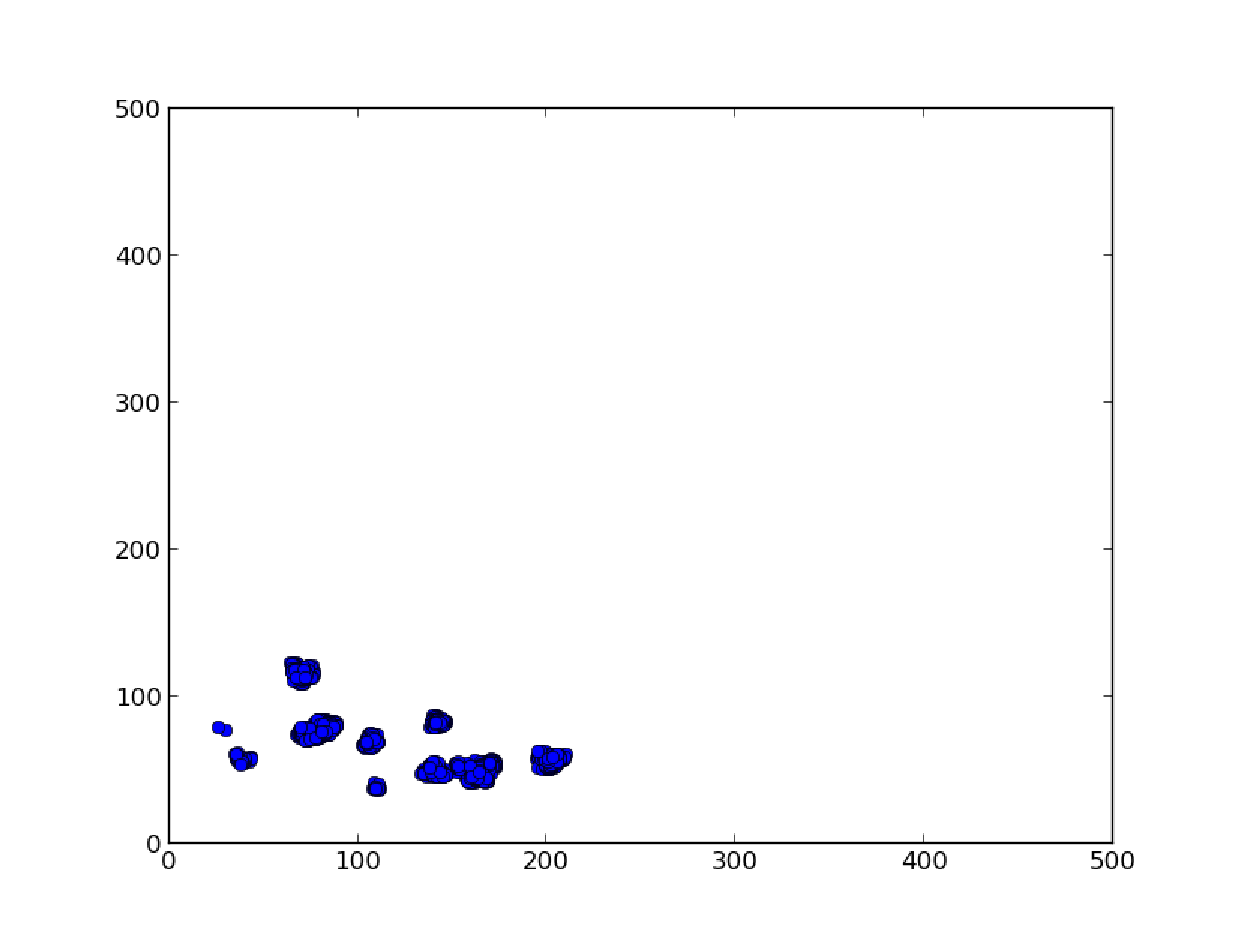
\includegraphics[width=0.9\textwidth]{figures/chap5/attack-mobile-5iterations.eps}\label{fig:mobile-5queries}
\end{minipage}
}
\hfill
\subfigure[10次查询后]
{
\begin{minipage}[b]{0.45\textwidth}
  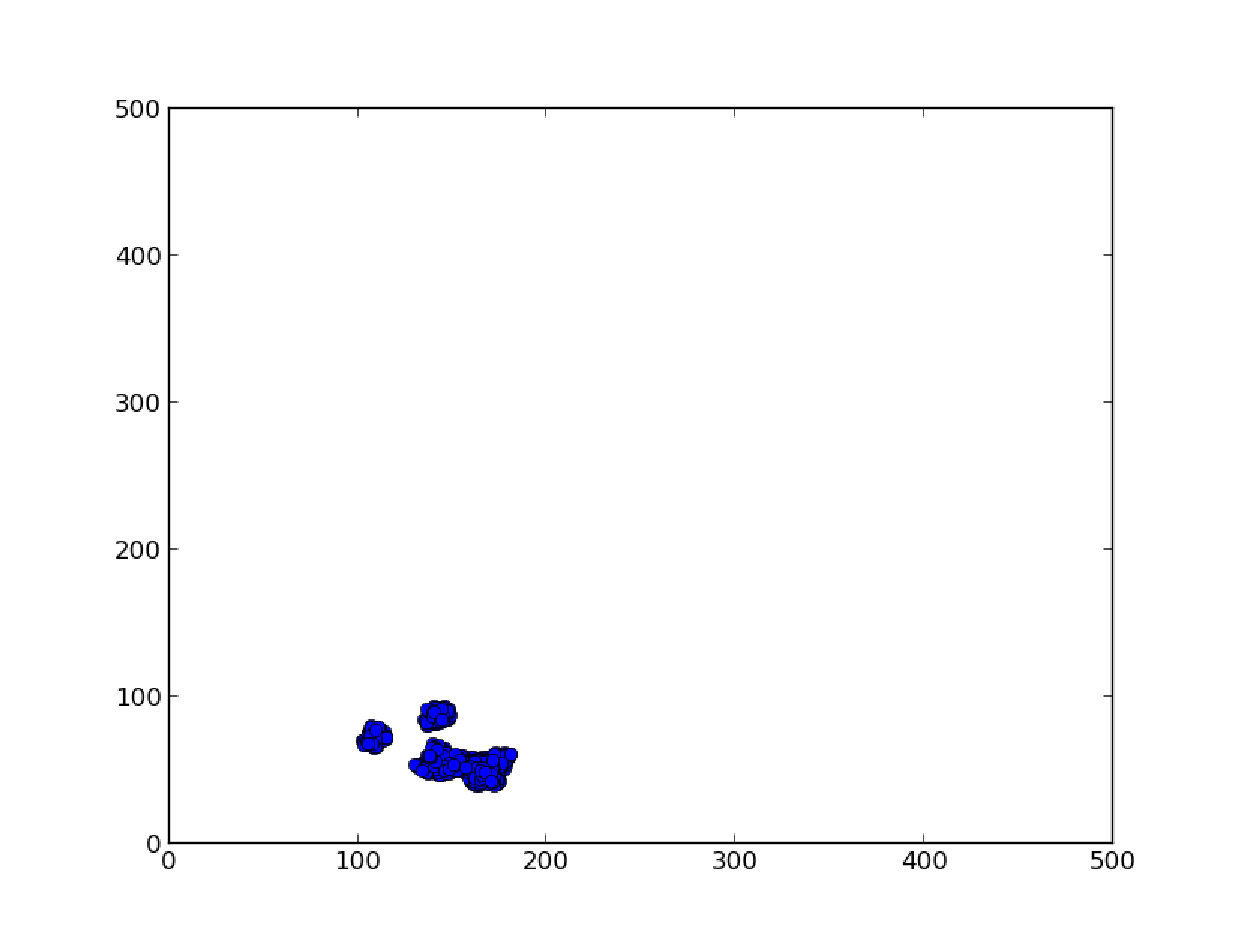
\includegraphics[width=0.9\textwidth]{figures/chap5/attack-mobile-10iterations.eps}\label{fig:mobile-10queries}
\end{minipage}
}

\subfigure[15次查询后]
{
\begin{minipage}[b]{0.45\textwidth}
  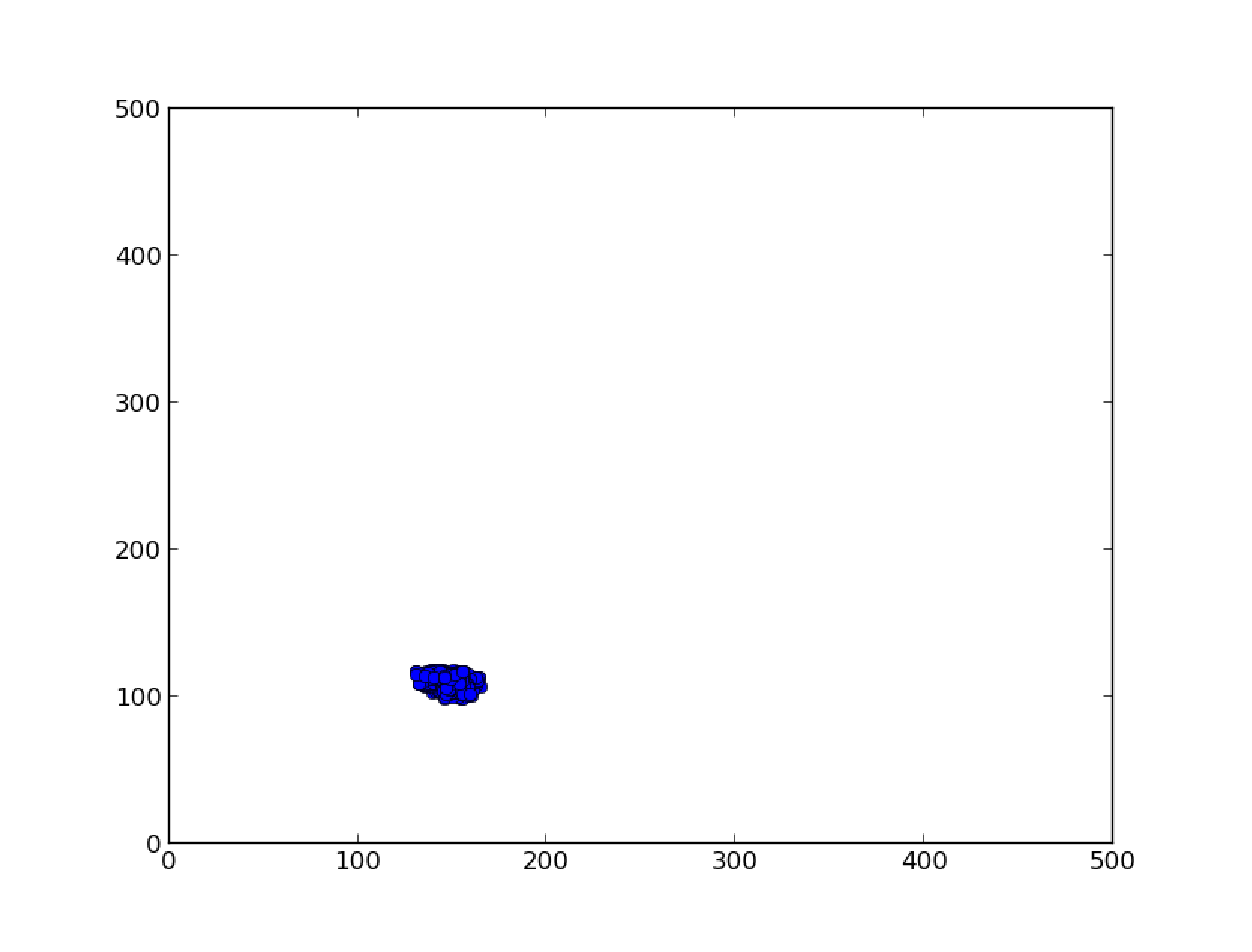
\includegraphics[width=0.9\textwidth]{figures/chap5/attack-mobile-15iterations.eps}\label{fig:mobile-15queries}
\end{minipage}
}
\hfill
\subfigure[20次查询后]
{
\begin{minipage}[b]{0.45\textwidth}
  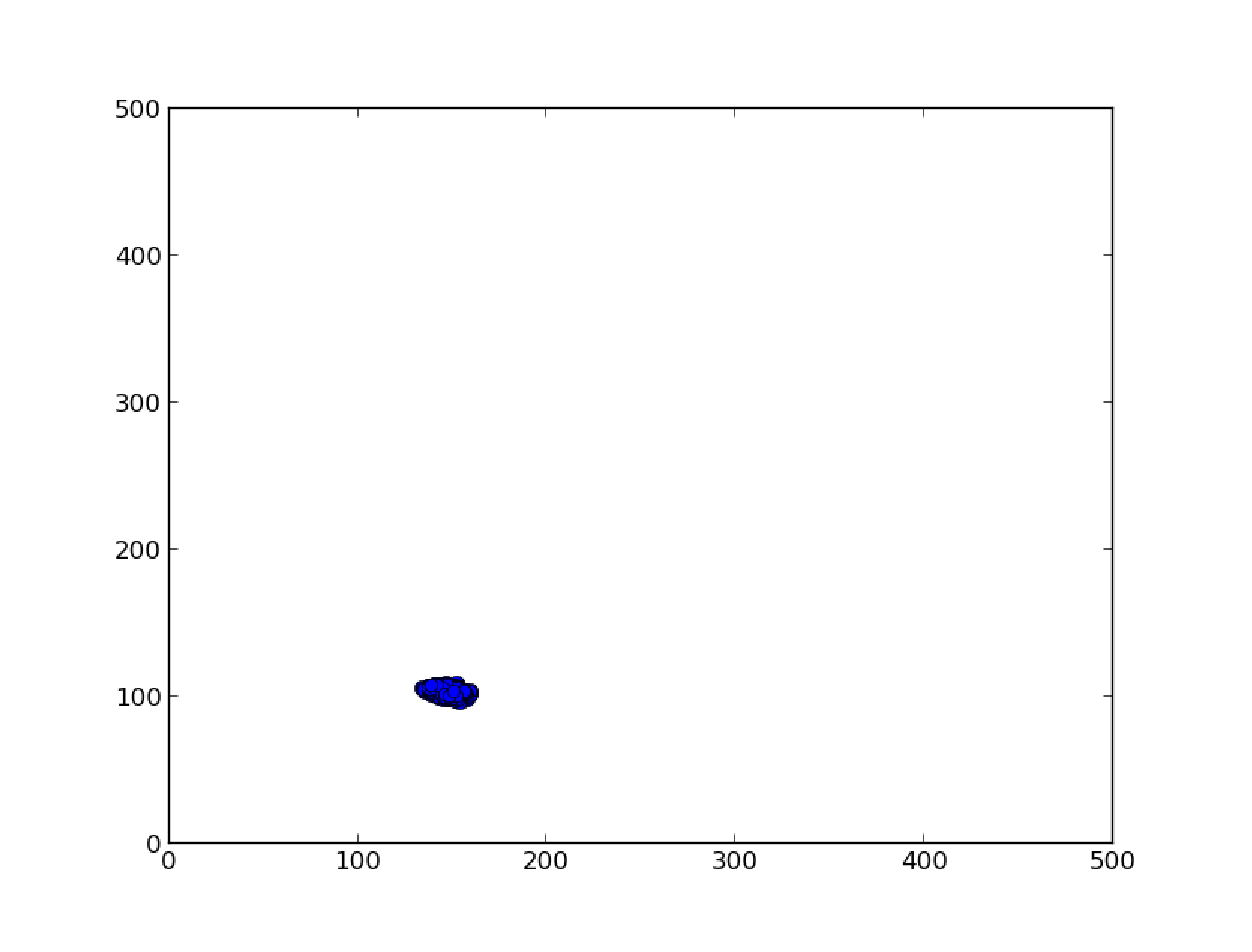
\includegraphics[width=0.9\textwidth]{figures/chap5/attack-mobile-20iterations.eps}\label{fig:mobile-20queries}
\end{minipage}
}
\caption{跟踪过程中的粒子位置状态}\label{fig:particles}
\end{figure}

一般情况下,我们仅通过20次查询即可将移动的认知用户位置锁定在较小的区域范围内。进一步,为了衡量跟踪的准确程度,我们采用第\ref{chap:fixed}章提出的平均误差距离的概念来对文中提出的跟踪算法进行准确性的描述。我们对几种不同的运动形式包括直线运动、一般形式的曲线运动、以及随机游动分别进行了对比,如图\ref{fig:diverse-pattern}所示。其中实验结果表明,我们提出的算法对几种不同的运动方式都有比较好的跟踪精确度,而且对于不同运动状态的移动用户的跟踪结果相差无几。随着时间以及查询次数的增加,对目标认知用户的跟踪精度也逐渐增加。

\begin{figure}[!htp]\label{fig:diverse-pattern}
  \centering
  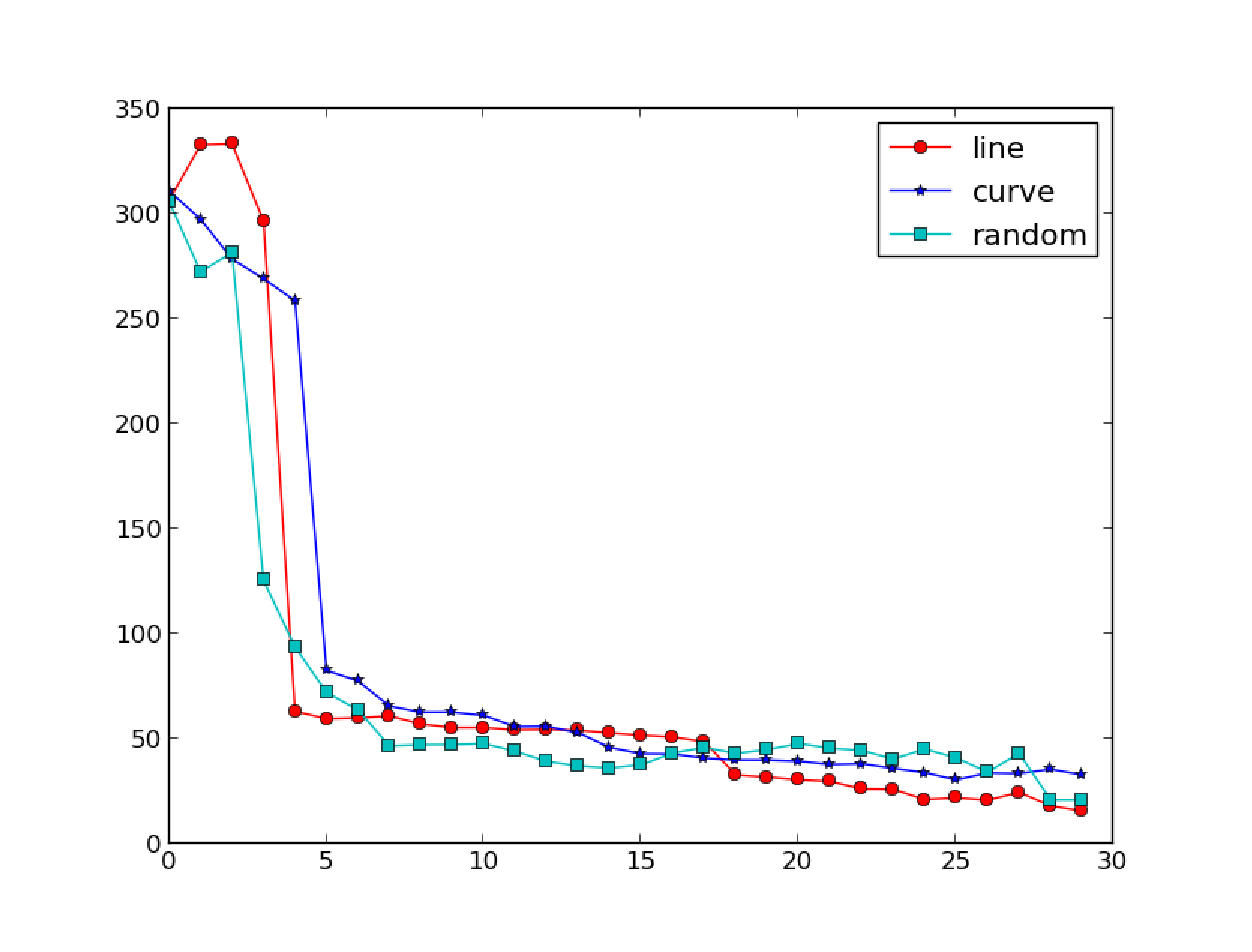
\includegraphics[width=0.7\textwidth]{figures/chap5/diversity}\bicaption[fig:diverse-pattern]{对不同运动形式用户的跟踪结果}{对不同运动形式用户的跟踪结果}{Fig}{Tracking Results on Mobile Users of Different Patterns}
\end{figure}

为检验提出的隐私保护的频谱查询和使用方案的有效性,我们对20组实验数据进行了统计,每一次实验随机生成主用户的位置并随机设置认知用户的移动轨迹。我们将采用隐私保护频谱查询和选择方案前后的跟踪误差进行了对比,如图\ref{fig:countermeasure}所示。容易看出,在使用隐私保护的频谱查询和选择方案后,由于认知用户在运动过程中尽可能选择功率大且覆盖范围广的频谱资源,而且尽量减少不必要的频道切换,导致
攻击者在短期内几乎无法通过本文提出的算法实现跟踪,攻击效率大幅度下降。

\begin{figure}[!htp]\label{fig:countermeasure}
  \centering
  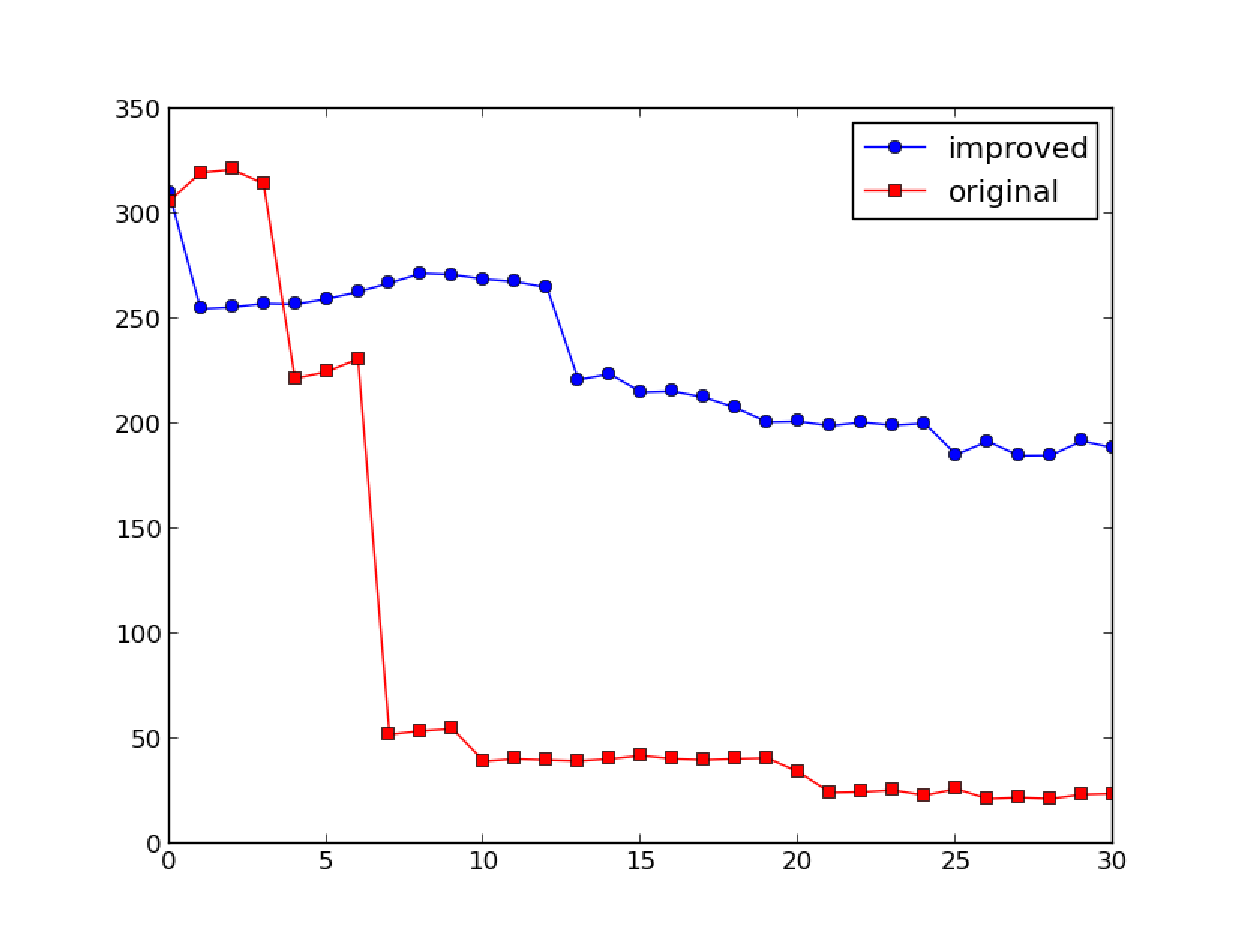
\includegraphics[width=0.7\textwidth]{figures/chap5/countermeasure}\bicaption[fig:countermeasure]{隐私保护的查询和选择方案的性能}{隐私保护的查询和选择方案的性能}{Fig}{Performance of Privacy Preserving Spectrum Query and Selection Scheme}
\end{figure}